%% LyX 1.1 created this file.  For more info, see http://www.lyx.org/.
%% Do not edit unless you really know what you are doing.
\documentclass[english]{amsart}
\usepackage[T1]{fontenc}
\usepackage[latin1]{inputenc}
\usepackage{babel}
\usepackage{graphics}

\makeatletter

%%%%%%%%%%%%%%%%%%%%%%%%%%%%%% LyX specific LaTeX commands.
\providecommand{\LyX}{L\kern-.1667em\lower.25em\hbox{Y}\kern-.125emX\@}

%%%%%%%%%%%%%%%%%%%%%%%%%%%%%% Textclass specific LaTeX commands.
 \theoremstyle{plain}    
 \newtheorem{thm}{Theorem}[section]
 \numberwithin{equation}{section} %% Comment out for sequentially-numbered
 \numberwithin{figure}{section} %% Comment out for sequentially-numbered
 \theoremstyle{plain}    
 \newtheorem{lem}[thm]{Lemma} %%Delete [thm] to re-start numbering
 \theoremstyle{plain}    
 \newtheorem{prop}[thm]{Proposition} %%Delete [thm] to re-start numbering
 \theoremstyle{plain}    
 \newtheorem{algorithm}[thm]{Algorithm} %%Delete [thm] to re-start numbering

%%%%%%%%%%%%%%%%%%%%%%%%%%%%%% User specified LaTeX commands.
\newcommand{\R}{{\sf R\hspace*{-0.9ex}\rule{0.15ex}%
       {1.3ex}\hspace*{0.9ex}}}
\newcommand{\N}{{\sf N\hspace*{-1.0ex}\rule{0.15ex}%
       {1.1ex}\hspace*{1.0ex}}}
\newcommand{\Q}{{\sf Q\hspace*{-1ex}\rule{0.15ex}%
       {1.3ex}\hspace*{1.1ex}}}
\newcommand{\C}{{\sf C\hspace*{-0.9ex}\rule{0.15ex}%
       {1.3ex}\hspace*{0.9ex}}}
\usepackage{epsfig}
\usepackage{amsmath,amssymb}
\usepackage{pslatex}
\usepackage{color}


\newif \ifpdf
    \ifx \pdfoutput \undefined
        \pdffalse
    \else
        \pdftrue
\fi


\ifpdf
 \usepackage{thumbpdf}
 \usepackage[pdftex,urlcolor=black,colorlinks=false]{hyperref}
 \pdfinfo{
            /Title      (A family of 4-points dyadic high resolution subdivision schemes)
            /Author     (Daniel Lemire, Ph.D.)
            /Subject 	( By using temporary placeholders on a dense grid, we generalize the 4-point dyadic cubic Deslauriers-Dubuc scheme. Interpolated values require 2 steps to stabilize as they are first interpolated on a coarse scale through a tetradic filter and then on a finer scale using a dyadic filter. The interpolants are C^{1} and can be chosen to reproduce polynomials of degree 4. These generalized interpolatory subdivision schemes have minimal support and no additional memory requirement. This work has applications in CAGD and wavelet theory.)
            /Keywords   (subdivision schemes, interpolation, CAGD, wavelets)
          }

\else
    \usepackage[ps2pdf]{hyperref}
\fi

\topmargin  = 0pt
\headheight = 0pt
\headsep    = 0pt

\voffset    = 0in
\hoffset    = 0in
\textheight = 230mm
\textwidth  = 164mm

\evensidemargin = 0pt
\oddsidemargin  = 0pt

\pagestyle{empty}
\usepackage{float}

\definecolor{veryblackblue}{rgb}{0.0,0.0,0.1}

%% Background of blue palette
 \definecolor{webblackblue}{rgb}{0.0,0.0,0.2}
 \definecolor{webblue}{rgb}{0.0, 0.0, 0.6}

%% Background of red palette
 \definecolor{webblackred}{rgb}{0.2,0.0,0.0}
 \definecolor{webred}{rgb}{0.6,0.0,0.0}

%% Background of green palette
 \definecolor{webblackgreen}{rgb}{0.0,0.2,0.0}                                   
 \definecolor{webgreen}{rgb}{0.0,0.6,0.0} 

%% Background of magenta palette
 \definecolor{webblackmagenta}{rgb}{0.14,0.0,0.14}                                   
 \definecolor{webmagenta}{rgb}{0.42,0.0,0.42} 

%% Background of cyan palette
 \definecolor{webblackcyan}{rgb}{0.0,0.14,0.14}                                   
 \definecolor{webcyan}{rgb}{0.0,0.42,0.42} 

%% Background of yellow pallete
 \definecolor{webblackyellow}{rgb}{0.14,0.14,0.0}                                   
 \definecolor{webyellow}{rgb}{0.85,0.85,0.0} 

 \definecolor{webdarkgray}{rgb}{0.2,0.2,0.2}

 \definecolor{webgray}{rgb}{0.75,0.75,0.75}
 \definecolor{weborange}{rgb}{1.0, 0.6, 0.0}

\renewcommand\labelenumi{\textcolor{webdarkgray}{\arabic{enumi}.}}
\newcommand{\setenumi}[1]{#1.\setcounter{enumi}{#1}}
\usepackage{dsfont}

\makeatother
\begin{document}

\title{A Family of 4-point Dyadic High Resolution Subdivision Schemes}


\author{Daniel Lemire}

\begin{abstract}
By using temporary placeholders on a dense grid, we generalize the
4-point dyadic cubic Deslauriers-Dubuc scheme. Interpolated values
require 2 steps to stabilize as they are first interpolated on a coarse
scale through a tetradic filter and then on a finer scale using a
dyadic filter. The interpolants are \( C^{1} \) and can be chosen
to reproduce polynomials of degree 4. These generalized interpolatory
subdivision schemes have minimal support and no additional memory
requirement. This work has applications in CAGD and wavelet theory.
\end{abstract}

\keywords{Subdivision Schemes, Fourier transform, CAGD, Wavelets, Lagrange
Interpolation}

\maketitle

\section{Introduction}

Interpolatory subdivision schemes interpolate a discrete set of data
points in a local manner, that is, the value of the interpolation
function at a given point depends on a small number of nearby data
points. The classical dyadic algorithm introduced by Deslauriers and
Dubuc \cite{Du,DeDu} finds the midpoint values by fitting a Lagrange
polynomial through the \( 2N \) closest data points. By repeating
this algorithm again and again, each time doubling the number of data
points or nodes by midpoint interpolation, we eventually have a dense
set of data points and we can determine uniquely a smooth interpolation
function. Because interpolatory subdivision schemes relate data points
from one scale to the data points at another scale, it is not surprising
that they are a key ingredient in the construction of compactly supported
wavelets \cite{Dau,DeDuLe}.

More recently, Merrien \cite{Me92,Me99,DuLeMe} introduced Hermite
subdivision schemes. Since Merrien subdivision schemes use Hermite
nodes, they have have twice the approximation order and better regularity
for a given support. For example \( 2- \)point Hermite schemes are
differentiable and can reproduce quadratic or cubic polynomials whereas
the corresponding Deslauriers-Dubuc scheme (the linear spline) isn't
differentiable and can only reproduce linear polynomials. 

Since Deslauriers-Dubuc schemes have important applications, it is
tempting to add extra nodes to Deslauriers and Dubuc schemes as an
attempt to improve them to get {}``high resolution'' schemes. Doubling
the number of nodes is costly effectively doubling the memory requirements,
however, since a dyadic subdivision scheme doubles its memory usage
at each step, we can choose to use right away this upcoming extra
storage space without any cost. In effect, we can simply make use
of the memory that will be allocated later in any case. Therefore,
we can freely increase the number of nodes in intermediate steps.
These new placeholders can then be used to record a coarse scale guess
(using a tetradic filter) which we can later combine with a finer
scale interpolation (using a dyadic filter). As a special case, we
may choose to ignore the coarse scale estimate, in which case our
approach amounts to a Deslauriers-Dubuc scheme; we can also use this
approach to reproduce polynomials of degree \( 4 \) by a Richardson
extrapolation approach. The main result of this paper is that by summing
up the tetradic (coarse) interpolation recorded in placeholders and
dyadic (fine) interpolations, we get a range of smooth (\( C^{1} \))
high resolutions schemes reproducing cubic polynomials.


\section{Subdivision schemes}

Interpolatory subdivision schemes where first introduced by Deslauriers
and Dubuc (quote). Let \( b>1 \) be an integer, given two integers
\( k,j \), the number \( x_{j,k}=k/b^{j} \) is said to be \( b- \)adic
(of depth \( j \)). For a fixed \( j \), the \( b- \)adic numbers
form a regularly spaced set of nodes. Given some data \( \left\{ y_{J,k}\right\} _{k\in \N } \)
on the \( b- \)adic numbers of depth \( J \), we want to build a
smooth fonction \( f \) such that \( f\left( x_{J,k}\right) =y_{J,k}\, \forall k\in \N  \).
Starting with this initial data (\( y_{J,k} \)) and using the linear
formula \begin{equation}
\label{basicsubdivision}
y_{j+1,l}=\sum _{k\in \N }\gamma _{bk-l}y_{j,k}
\end{equation}
 for some constant array \( \gamma  \), we get values \( y_{J,k} \)
for any \( j>J \) and since \( b- \)adic numbers form a dense set
of the real numbers, there is at most one continuous function such
that \( f\left( x_{j,k}\right) =y_{j,k} \) for all \( k,j>J \). 

A subdivision scheme is interpolatory and will satisfy \( f\left( x_{J,k}\right) =y_{J,k} \)
if \( \gamma _{bk}=0 \) except when \( k=0 \). We say that a subdivision
scheme is stationary if the array \( \gamma  \) is constant (doesn't
depend on \( j \)). An interpolatory subdivision scheme is said to
be \( 2N- \)point if \( \gamma _{l}=0 \) for \( |l|>Nb \). The
interpolation function \( f \) computed from a \( 2N- \)point \( b- \)adic
scheme with initial data \( y_{0,0}=1 \) and \( y_{0,k}=0 \) for
all \( k\neq 0 \) is said to be the fundamental function and has
a compact support of \( [-(Nb-1)/(b-1),(Nb-1)/(b-1)] \) or \( [1-2N,2N-1] \)
when \( b=2 \). Hence as \( N \) increases the support of the fundamental
function increases.

For \( N=1,2,3,... \) there are corresponding \( 2N- \)point interpolatory
Deslauriers-Dubuc subdivision schemes and they are built from the
midpoint evaluation of Lagrange polynomial of degree \( 2N-1 \).
For \( b=2 \) (dyadic case), the \( 4- \)point Deslauriers-Dubuc
scheme can be defined by the array \( \gamma ^{DD2} \) given by \( \gamma _{0}^{DD2}=1,\,  \)\( \gamma _{1}^{DD2}=\gamma ^{DD2}_{-1}=-9/16,\,  \)\( \gamma _{3}^{DD2}=\gamma _{-3}^{DD2}=-1/16 \)
with \( \gamma _{k}^{DD2}=0 \) otherwise; for \( b=4 \) (tetradic
case), the scheme is defined by \( \gamma ^{DD4} \) given by \( \gamma _{2k}^{DD4}=\gamma ^{DD2}_{k}\, \forall k\in \N ,\,  \)
\( \gamma _{-1}^{DD4}=\gamma _{1}^{DD4}=105/128,\,  \)\( \gamma _{-3}^{DD4}=\gamma _{-3}^{DD4}=35/128,\,  \)\( \gamma _{-5}^{DD4}=\gamma _{5}^{DD4}=-7/128,\,  \)\( \gamma _{-7}^{DD4}=\gamma _{7}^{DD4}=-5/128,\,  \)with
\( \gamma _{k}^{DD2}=0 \) otherwise. Because \( 4- \)point Deslauriers-Dubuc
schemes are derived from cubic Lagrange polynomials, they reproduce
cubic polynomials, that is, if the initial data \( y_{j,k} \) satisfies
\( y_{j,k}=p\left( x_{j,k}\right) \, \forall k\in \N  \) for some
cubic polynomial \( p \) then the interpolation function \( f \)
is this same cubic polynomial \( f=p \). The two cases presented
above (\( \gamma ^{DD2} \) and \( \gamma ^{DD4} \)) reproduce cubic
polynomials and it can also be shown that they both give differentiable
(\( C^{1} \)) interpolation functions. Because we later borrow from
these two subdivision schemes, we give explicit algorithms for both
schemes.

\begin{algorithm}
(\( 4- \)point Deslauriers-Dubuc Dyadic Scheme) The following iteration
steps depend on \( \alpha  \), a constant parameter.
\begin{enumerate}
\item recopy data for \( x_{j,k}=x_{j+1,2k} \): \( y_{j+1,2k}=y_{j,k}\, \forall k\in \N  \)
;
\item interpolate midpoint value by the corresponding cubic Lagrange polynomial:
\[
y_{j+1,2k+1}=\frac{-y_{j,k-1}+9y_{j,k}+9y_{j,k+1}-y_{j,k+2}}{128}\, \forall k\in \N ;\]

\item Repeat with \( j\rightarrow j+1 \) and using \( y_{j+1} \) as initial
data.
\end{enumerate}
\end{algorithm}
~

\begin{algorithm}
(\( 4- \)point Deslauriers-Dubuc Tetradic Subdivision Scheme) The
following iteration steps depend on \( \alpha  \), a constant parameter.
\begin{enumerate}
\item recopy data for \( x_{j,k}=x_{j+1,2k} \): \( y_{j+1,4k}=y_{j,k}\, \forall k\in \N  \)
;
\item interpolate quartertile point values by the corresponding cubic Lagrange
polynomial: \[
y_{j+1,4k+1}=\frac{-7y_{j,k-1}+105y_{j,k}+35y_{j,k+1}-5y_{j,k+2}}{128};\]
 \[
y_{j+1,2k+1}=\frac{-y_{j,k-1}+9y_{j,k}+9y_{j,k+1}-y_{j,k+2}}{128};\]
\[
y_{j+1,4k+3}=\frac{-5y_{j,k-1}+35y_{j,k}+105y_{j,k+1}-7y_{j,k+2}}{128}\, \forall k\in \N ;\]

\item Repeat with \( j\rightarrow j+1 \) and using \( y_{j+1} \) as initial
data.
\end{enumerate}
\end{algorithm}

\subsection{Approximation order for subdivision schemes}

We are interested in measuring how well a given subdivsion scheme
can approximation functions. One such measure is given by the approximation
order of the scheme \cite[definition 2]{KuVD98}. We say that a subdivision
scheme has approximation order \( p \) if given given any smooth
function \( g\in C^{p}\left( \left[ 0,1\right] \right)  \), the interpolation
function \( f \) satisfying \( f\left( x_{j,k}\right) =g\left( x_{j,k}\right) \, \forall k\in \N  \)
is such that \( \left\Vert f-g\right\Vert _{L^{\infty }\left( \left[ 0,1\right] \right) }\leq C/b^{jp} \)
for a constant \( C \) independent of \( j \).

For a continuous subdivision scheme reproducing polynomials of degree
\( p \), it is sufficient for the scheme to converge to a continous
function to have approximation order \( p+1 \) \cite{KuVD98}. Specifically,
this means that \( 4- \)point Deslauriers-Dubuc schemes have approximation
order \( 4 \).


\section{High resolution subdivsion schemes}


\subsection{Definitions}

In this paper, we want to show how the subdivision scheme framework
can be extended to build hybrid schemes: mixing tetradic and dyadic
subdivision schemes for example. Given some data \( \left\{ y_{j-1,k}\right\} _{k\in \N } \)
to interpolate on the \( x_{j-1,k} \) grid, we first apply a dyadic
subdivision scheme such as the \( 4- \)point Deslauriers-Dubuc scheme
to get finer scale data \( y_{j,k} \). For any \( j' \), the odd
nodes \( y_{j',2k+1} \)will be referred to as {}``placeholders''
because their assigned value will change in general whereas the even
nodes are referred to as stable that is, we require \( y_{j+1,4k}=y_{j,2k}\, \forall k\in \N  \)
but not \( y_{j+1,4k+2}=y_{j,2k+1} \). Hence the purpose of first
applying a dyadic subdivision scheme is to fill the placeholders (\( y_{j,2k+1} \)).
With this setting, the following algorithm is interpolatory.

\begin{algorithm}
\label{4pointhrssalgo}(\( 4- \)point Dyadic High Resolution Subdivision
Scheme) The following iteration steps depend on \( \alpha  \), a
constant parameter.
\begin{enumerate}
\item recopy stable data: \( y_{j+1,4k}=y_{j,2k}\, \forall k\in \N  \)
;
\item Apply the \( 4- \)point Deslauriers-Dubuc tetradic scheme on even
(stable) nodes: \[
y_{j+1,4k+1}=\frac{-7y_{j,2k-2}+105y_{j,2k}+35y_{j,2k+2}-5y_{j,2k+4}}{128};\]
 \[
y_{j+1,4k+2}^{temporary}=\frac{-y_{j,2k-2}+9y_{j,2k}+9y_{j,2k+2}-y_{j,2k+4}}{128};\]
\[
y_{j+1,4k+3}=\frac{-5y_{j,2k-2}+35y_{j,2k}+105y_{j,2k+2}-7y_{j,2k+4}}{128}\, \forall k\in \N ;\]

\item Update midpoint (which then becomes stable): \[
y_{j+1,4k+2}=(1-\alpha )y_{j+1,4k+2}^{temporary}+\alpha y_{j,2k+1};\]

\item Repeat with \( j\rightarrow j+1 \) and using \( y_{j+1} \) as initial
data.
\end{enumerate}
\end{algorithm}
This new algorithm is not a subdivision scheme and thus we need to
propose a more general definition: subdivision schemes (equation \ref{basicsubdivision})
can be generalized by the linear equation\begin{equation}
\label{hrgeneral}
y_{j+1,l}=\sum _{m=1}^{M}\sum _{k\in \N }\gamma _{Nbk+m-1-l}^{(m)}y_{j,Nk+m-1}
\end{equation}
where \( \gamma ^{(1)},...,\gamma ^{(M)} \) are constant arrays (independent
from \( j \)). It can be said to be \( b- \)adic because the number
of nodes is increasing by a factor of \( b \) with each iteration
but because we have \( M \) arrays \( \gamma  \), the scheme is
said to be a high resolution subdivision scheme if \( M>1 \). For
\( b=M=2 \) the general equation \ref{hrgeneral} becomes \begin{equation}
\label{N2highres}
y_{j+1,l}=\sum _{k\in \N }\gamma _{4k-l}^{(1)}y_{j,2k}+\gamma _{4k+1-l}^{(2)}y_{j,2k+1}.
\end{equation}
Algorithm \ref{4pointhrssalgo} amounts to choosing \( \gamma ^{(1)} \)
and \( \gamma ^{(2)} \) to be:

\begin{eqnarray}
\gamma ^{(1)}_{2k}=\gamma _{2k}^{DD4}+\alpha \left( \delta _{k,0}-\gamma _{k}^{DD2}\right) ,\,  & \gamma _{2k+1}^{(1)}=\gamma _{2k+1}^{DD4}\, \forall k\in \N  & \label{N2highres_1} \\
\gamma ^{(2)}_{0}=\alpha ,\,  & \gamma ^{(2)}_{k}=0\, otherwise\label{N2highres_2} 
\end{eqnarray}
 for some parameter \( \alpha \in \R  \). 

In the simplest case, \( \alpha =0 \), equation \ref{N2highres}becomes\begin{equation}
\label{N2highresalpha0}
y_{j+1,l}=\sum _{k\in \N }\gamma ^{DD4}_{4k-l}y_{j,2k}.
\end{equation}
Because \( \gamma ^{(2)}=0 \) in this case, we see that the placeholders
(odd nodes) are effectively ignored. Indeed, we observe that this
last equation discards odd nodes at each step: \( y_{j+1,l} \) depends
only on even nodes (\( y_{j,2k} \) ) and not at all on the odd nodes
( \( y_{j,2k+1} \)). Hence, we can replace equation \ref{N2highresalpha0}
by \[
y_{j+1,2l}=\sum _{k\in \N }\gamma ^{DD4}_{4k-2l}y_{j,2k}\]
but because \( \gamma _{2k}^{DD4}=\gamma ^{DD2}_{k} \) , this last
equation becomes \( y_{j+1,2l}=\gamma ^{DD2}_{2k-l}y_{j,2k} \) and
if we define \( \widetilde{y}_{j,k}=y_{j,2k} \) then \begin{equation}
\label{DD2}
\widetilde{y}_{j+1,2l}=\sum _{k\in \N }\gamma ^{DD2}_{2k-l}\widetilde{y}_{j,2k}
\end{equation}
which we recognize as the cubic Deslauriers-Dubuc scheme. We could
also show the same result by looking at algorithm \ref{4pointhrssalgo}.

\begin{prop}
\label{propDesDuequiv}For \( \alpha =0 \), the high resolution scheme
given by algorithm \ref{4pointhrssalgo} (or equations \ref{N2highres},
\ref{N2highres_1}, and \ref{N2highres_2}) is equivalent to the \( 4- \)point
dyadic Deslauriers-Dubuc subdivision scheme (discarding the odd nodes
or placeholders in the first iteration).
\end{prop}
In general, since \( \gamma _{2k}^{DD4}=\gamma ^{DD2}_{k} \), we
can rewrite equation \ref{N2highres} for even and odd terms. Firstly,
setting \( l=2s \) (\( l \) even), we have \begin{eqnarray*}
y_{j+1,2s} & =\sum _{k\in \N } & \gamma _{4k-2s}^{(1)}y_{j,2k}+\gamma _{4k+1-2s}^{(2)}y_{j,2k+1}\\
 & =\sum _{k\in \N } & \left( \gamma ^{DD4}_{4k-2s}-\alpha \gamma ^{DD2}_{2k-s}+\alpha \delta _{4k,2s}\right) y_{j,2k}+\alpha \delta _{4k+1,s}y_{j,2k+1}\\
 & =\sum _{k\in \N } & \left( (1-\alpha )\gamma ^{DD2}_{2k-s}+\alpha \delta _{2k,s}\right) y_{j,2k}+\delta _{2k+1,s+1}\alpha y_{j,2k+1}
\end{eqnarray*}
so that when \( s \) is even (\( l=2s=4r \)), we have the interpolatory
condition \begin{equation}
\label{hrsinterpole}
y_{j+1,4r}=y_{j,2r}
\end{equation}
otherwise, when \( s \) is odd \( (l=2s=4r+2) \)\begin{equation}
\label{hrsricharson}
y_{j+1,4r+2}=\alpha y_{j,2r+1}+(1-\alpha )\sum _{k\in \N }\gamma ^{DD2}_{2k-2r-1}y_{j,2k}.
\end{equation}
Secondly, if \( l \) is odd (\( l=2s+1 \)), we have\begin{eqnarray}
y_{j+1,2s+1} & = & \sum _{k\in \N }\gamma _{4k-2s-1}^{(1)}y_{j,2k}+\gamma _{4k-2s-1}^{(2)}y_{j,2k+1}\nonumber \\
 & = & \sum _{k\in \N }\gamma ^{DD4}_{4k-2s-1}y_{j,2k}.\label{hrswidguess} 
\end{eqnarray}
Equations \ref{hrsinterpole}, \ref{hrsricharson}, and \ref{hrswidguess}
can be used to describe the chosen high resolution schemes: while
equation \ref{hrsinterpole} is the interpolatory condition, equation
\ref{hrswidguess} fills the placeholders with tetradic (coarse scale)
interpolated values whereas equation \ref{hrsricharson} combines
the value stored in the placeholder with the newly available interpolated
value (fine scale) given by the summation term which we recognize
from the dyadic Deslauriers-Dubuc interpolation. 


\subsection{Reproduced polynomials}

Assume that for some \( j \), \( y_{j,k}=p_{3}\left( x_{j,k}\right)  \)
for some cubic polynomial \( p_{3} \), because \( 4- \)point Deslauriers-Dubuc
schemes reproduce cubic polynomials, we have \[
\sum _{k\in \N }\gamma ^{DD2}_{2k-2r-1}y_{j,2k}=y_{j,2r+1}=p_{3}\left( x_{j,2r+1}\right) \]
and thus equation \ref{hrsricharson} becomes \( y_{j+1,4r+2}=p_{3}\left( x_{j,2r+1}\right)  \)
. Similarly, equation \ref{hrswidguess} implies \( y_{j+1,2s+1}=p_{3}\left( x_{j+1,2s+1}\right)  \).
We can conclude that \( y_{j+1,k}=p_{3}\left( x_{j+1,k}\right)  \)
if \( y_{j,k}=p_{3}\left( x_{j,k}\right)  \) and thus the high resolution
scheme reproduce cubic polynomials. For practical implementations
of a high subdivision scheme, it is necessary to first apply a one-step
subdivision scheme since in general, we don't have placeholder values
precomputed. As we've seen this can be solved by a one-step dyadic
Deslauriers-Dubuc interpolation. Let \( \left\{ y_{j,k}\right\} _{k} \)
be some initial data. As a first step, we apply equation\begin{equation}
\label{DD2_2}
y_{j+1,l}=\sum _{k\in \N }\gamma ^{DD2}_{2k-l}y_{j,2k}
\end{equation}
 followed by equation \ref{N2highres} with \( j=j+1 \), and so on
(we follow algorithm \ref{4pointhrssalgo}). By induction, we get
the following lemma.

\begin{lem}
High resolution schemes given by algorithm \ref{4pointhrssalgo} (or
equations \ref{N2highres}, \ref{N2highres_1}, and \ref{N2highres_2})
using a one step 4-point dyadic Deslauriers-Dubuc interpolation (equation
\ref{DD2_2}) as an initialization step reproduce cubic polynomials.
\end{lem}
We can also get a stronger result by choosing a specific \( \alpha  \).
Let \( p_{4}(x)=a_{4}x^{4}+p_{3}(x) \) where \( p_{3} \) is some
cubic polynomial. Suppose that for some \( j \), \( y_{j,2k}=p_{4}\left( x_{j,2k}\right) ,\, y_{j-1,k}=p_{4}\left( x_{j-1,k}\right) \, \forall k\in \N  \).
We can write \( y_{j+1,4r+2} \) in terms of this initial data (\( y_{j} \)
and \( y_{j-1} \)) by substituting equation \ref{hrswidguess} into
\ref{hrsricharson} to get \begin{eqnarray}
y_{j+1,4r+2} & = & \alpha y_{j,2r+1}+(1-\alpha )\sum _{k\in \N }\gamma ^{DD2}_{2k-2r-1}y_{j,2k}\nonumber \\
 & = & \alpha \sum _{k\in \N }\gamma ^{DD4}_{4k-2r-1}y_{j-1,2k}+(1-\alpha )\sum _{k\in \N }\gamma ^{DD2}_{2k-2r-1}y_{j,2k}.\label{upcomingrichardson} 
\end{eqnarray}
We want to show that \( y_{j+1,4r+2}=p_{4}\left( x_{j,2r+1}\right)  \)
for some \( \alpha  \) and so we substitute \( y_{j,2k}=p_{4}\left( x_{j,2k}\right) ,\, y_{j-1,k}=p_{4}\left( x_{j-1,k}\right) \, \forall k\in \N  \)
into the two sums of this last equation. Because of the easily verified
results \begin{eqnarray*}
\frac{-9}{2^{4j}} & = & \frac{-\left( x_{j,2r-2}\right) ^{4}+9\left( x_{j,2r}\right) ^{4}+9\left( x_{j,2r+2}\right) ^{4}-\left( x_{j,2r+4}\right) ^{4}}{128}-\left( x_{j,2r+1}\right) ^{4}\\
\frac{-105}{2^{4j}} & = & \frac{-7\left( x_{j,2r-4}\right) ^{4}+105\left( x_{j,2r}\right) ^{4}+35\left( x_{j,2r+4}\right) ^{4}-5\left( x_{j,2r+8}\right) ^{4}}{128}-\left( x_{j,2r+1}\right) ^{4}\\
 & = & \frac{-5\left( x_{j,2r-4}\right) ^{4}+35\left( x_{j,2r}\right) ^{4}+105\left( x_{j,2r+4}\right) ^{4}-7\left( x_{j,2r+8}\right) ^{4}}{128}-\left( x_{j,2r+1}\right) ^{4},
\end{eqnarray*}
we can compute each of the sums explicitely \begin{eqnarray*}
\sum _{k\in \N }\gamma ^{DD4}_{4k-2r-1}y_{j-1,2k} & = & p_{3}\left( x_{j,2r+1}\right) +a_{4}\sum _{k\in \N }\gamma ^{DD4}_{4k-2r-1}\times \left( x_{j-1,2k}=x_{j,4k}\right) ^{4}\\
 & = & p_{4}\left( x_{j,2r+1}\right) -\frac{105a_{4}}{2^{4j}}
\end{eqnarray*}
 and\begin{eqnarray*}
\sum _{k\in \N }\gamma ^{DD2}_{2k-2r-1}y_{j,2k} & = & p_{3}\left( x_{j,2r+1}\right) +a_{4}\sum _{k\in \N }\gamma ^{DD2}_{2k-2r-1}\times \left( x_{j,2k}\right) ^{4}\\
 & = & p_{4}\left( x_{j,2r+1}\right) -\frac{9a_{4}}{2^{4j}}
\end{eqnarray*}
Hence, setting \( \alpha =-3/32 \) in equation \ref{upcomingrichardson},
we get \[
y_{j+1,4r+2}=p_{4}\left( x_{j,2r+1}\right) -\frac{105\alpha +9(1-\alpha )}{2^{4j}}a_{4}=p_{4}\left( x_{j+1,4r+2}\right) \]
since for \( \alpha =-3/32 \), \( 105\alpha +9(1-\alpha )=0 \).
Therefore, the scheme reproduces polynomials of degree \( 4 \). 

Of course, this last result assumes that we initialize the data so
that \( y_{j,2k+1}=p_{4}\left( x_{j,2k+1}\right) -\frac{105a_{4}}{16\times 2^{4j}} \)
and \( y_{j,2k}=p_{4}\left( x_{j,2k}\right)  \) for all \( k\in \N  \).
We can get this result naturally by having \( y_{j-1,k}=p_{4}\left( x_{j,k}\right)  \)
and applying first the high resolution scheme (equation \ref{N2highres})
with \( \alpha =1 \) , since equations \ref{hrsinterpole} and \ref{hrsricharson}
will guarantee \( y_{j,2k}=p_{4}\left( x_{j,k}\right)  \) whereas
equation \ref{hrswidguess} will initialize the placeholders properly.
Indeed, the case \( \alpha =1 \) essentially relies only on the tetradic
interpolation and discard the finer scale guesses (dyadic). We have
show the following result.

\begin{prop}
For any given \( j \), if \( y_{j-1,k}=p_{4}\left( x_{j-1,k}\right)  \)
where \( p_{4} \) is a polynomial of degree \( 4 \) then applying
the high resolution scheme given by algorithm \ref{4pointhrssalgo}
(or equations \ref{N2highres}, \ref{N2highres_1}, and \ref{N2highres_2})
first with \( \alpha =1 \) as an initialization step and then with
\( \alpha =-3/32 \) will guarantee for the following iterations that
\( y_{j',2k}=p_{4}\left( x_{j',2k}\right)  \) for \( \forall k\in \N  \)
and all \( j'\geq j-1 \).
\end{prop}

\subsection{Sufficient conditions for regularity}

To study the regularity of high resolution schemes, it is convenient
rewrite formula \ref{N2highres} in terms of (trigonometric) polynomials.
Given some data \( y_{j,k} \), define \( P^{j}(z)=\sum _{k\in \N }y_{j,k}z^{k} \).
If \( P_{2}(z)=\sum _{k\in \N }\gamma _{k}^{DD2}z^{k} \), then the
equation of the \( 4- \)point dyadic Deslauriers-Dubuc scheme (equation
\ref{DD2_2}), can be rewritten \( P^{j+1}(z)=P_{2}(z)P^{j}(z^{2}) \).
Similarly, if \( P_{4}(z)=\sum _{k\in \N }\gamma _{k}^{DD4}z^{k} \),
then the tetradic subdivision scheme is given by \( P^{j+1}(z)=P_{4}(z)P^{j}(z^{2}) \).
\( \mathrm{I} \)t can be shown that we can rewrite the general equation
for high resolution subdivision schemes as \[
P^{j+1}(z)=\sum _{i=1}^{M}\Phi _{i}(z)P^{j}\left( e^{2\pi i/b}z^{b}\right) .\]
where \( \Gamma _{i} \) must be Laurent polynomials and similarly
for dyadic schemes (\( b=2 \)), \[
P^{j+1}(z)=\Phi _{1}(z)P^{j}\left( z^{2}\right) +\Phi _{2}(z)P^{j}\left( -z^{2}\right) .\]
 The equation of symbols for the \( 4- \)point cubic high resolution
sheme is (see equation \ref{N2highres} and algorithm \ref{4pointhrssalgo})\begin{eqnarray}
P^{j+1}(z) & = & \left\{ P_{4}\left( z\right) -\alpha P_{2}\left( z^{2}\right) +\alpha \right\} \left( \frac{P^{j}\left( z^{2}\right) +P^{j}\left( -z^{2}\right) }{2}\right) +\alpha \left( \frac{P^{j}\left( z^{2}\right) -P^{j}\left( -z^{2}\right) }{2}\right) \nonumber \\
 & = & \left\{ \frac{P_{4}\left( z\right) -\alpha P_{2}\left( z^{2}\right) }{2}+\alpha \right\} P^{j}\left( z^{2}\right) +\frac{P_{4}\left( z\right) -\alpha P_{2}\left( z^{2}\right) }{2}P^{j}\left( -z^{2}\right) \nonumber \\
 & = & \Gamma _{1}(z)P^{j}\left( z^{2}\right) +\Gamma _{2}(z)P^{j}\left( -z^{2}\right) .\label{gammas} 
\end{eqnarray}
Because \( \gamma _{2k}^{DD4}=\gamma ^{DD2}_{k}\, \forall k\in \N  \),
we observe that \( P_{2} \) is uneeded and everything can be written
in terms of \( P_{4} \), indeed \[
P_{4}\left( z\right) -\alpha P_{2}\left( z^{2}\right) =\frac{P_{4}\left( z\right) -P_{4}\left( -z\right) }{2}+(1-\alpha )\frac{P_{4}\left( z\right) +P_{4}\left( -z\right) }{2}\]
and thus, the symbols \( \Gamma _{1} \)and \( \Gamma _{2} \) can
be written \begin{eqnarray*}
\Gamma _{1}(z) & = & \Gamma _{2}(z)+\alpha \\
\Gamma _{2}(z) & = & \frac{P_{4}\left( z\right) -P_{4}\left( -z\right) }{4}+(1-\alpha )\frac{P_{4}\left( z\right) +P_{4}\left( -z\right) }{4}.
\end{eqnarray*}
When \( \alpha =0 \) (Deslauriers-Dubuc case), \( \Gamma _{1}(z)=\Gamma _{2}(z)=\frac{P_{4}\left( z\right) }{2} \)
and equation \ref{N2highres} becomes\[
P^{j+1}(z)=P_{4}\left( z\right) \left( \frac{P^{j}\left( z^{2}\right) +P^{j}\left( -z^{2}\right) }{2}\right) \]
and it can be shown to be equivalent to the Deslauriers-Dubuc dyadic
scheme by using the last equation for averaging \( P^{j+1}(z) \)
and \( P^{j+1}(-z) \), \begin{eqnarray*}
\frac{P^{j+1}(z)+P^{j+1}(-z)}{2} & = & \left( \frac{P_{4}\left( z\right) -P_{4}\left( -z\right) }{2}\right) \left( \frac{P^{j}\left( z^{2}\right) +P^{j}\left( -z^{2}\right) }{2}\right) \\
 & = & P_{2}\left( z^{2}\right) \left( \frac{P^{j}\left( z^{2}\right) +P^{j}\left( -z^{2}\right) }{2}\right) .
\end{eqnarray*}
which can be used to prove that when \( \alpha =0 \) the high resolution
subdivision scheme becomes the dyadic Deslauriers-Dubuc scheme (proposition
\ref{propDesDuequiv}).

In order to study the regularity and stability of the chosen high
resolution schemes, we need to find corresponding schemes for the
(forward) finite differences. Let \( dx_{j}=1/2^{j} \) and write
\[
D_{j,k}=\frac{dy_{j,k}}{dx_{j}}=2^{j}\left( y_{j,k+1}-y_{j,k}\right) ,\]
and define higher order finite differences recursively \[
D_{j,k}^{n}=d^{(n)}y_{j,k}/\left( dx_{j}\right) ^{n}=d\left( d^{(n-1)}y_{j,k}\right) /\left( dx_{j}\right) ^{n}=2^{jn}\times d^{(n)}y_{j,k}.\]
 Let \( H_{1}^{j} \) be the symbol for \( dy_{j,k}/dx_{j} \), then
\begin{eqnarray*}
H_{1}^{j}(z) & = & \sum _{k\in \N }2^{j}\left( y_{j,k+1}-y_{j,k}\right) z^{k}\\
 & = & \sum _{k\in \N }2^{j}y_{j,k}z^{k-1}-\sum _{k\in \N }2^{j}y_{j,k}z^{k}\\
 & = & 2^{j}(1/z-1)P^{j}(z)=2^{j}(1-z)P^{j}(z)/z,
\end{eqnarray*}
 and thus \( P^{j}\left( z^{2}\right) =z^{2}2^{j}H_{1}^{j}\left( z^{2}\right) /(1-z^{2}) \),
\( P^{j}\left( -z^{2}\right) =-z^{2}2^{j}H_{1}^{j}\left( -z^{2}\right) /(1+z^{2}) \),
and \( P^{j+1}(z)=z2^{j+1}H_{1}^{j+1}(z)/(1-z) \). Substituting these
three equations into \( P^{j+1}(z)=\Gamma _{1}(z)P^{j}\left( z^{2}\right) +\Gamma _{2}(z)P^{j}\left( -z^{2}\right)  \)
(equation \ref{gammas}) gives\[
H_{1}^{j+1}(z)=\frac{2z(1-z)}{(1-z^{2})}\Gamma _{1}(z)H_{1}^{j}\left( z^{2}\right) -\frac{2z(1-z)}{(1+z^{2})}\Gamma _{2}(z)H_{1}^{j}\left( -z^{2}\right) .\]
 Similarly, the higher order finite differences are given by\[
H_{n}^{j}(z)=\frac{2(1-z)}{z}H_{n-1}^{j}(z)=\left( \frac{2(1-z)}{z}\right) ^{n}P^{j}(z)\]
where \( H_{0}(z)=P(z) \) and it can be seen that they can be computed
by \begin{equation}
\label{genh}
H_{n}^{j+1}(z)=\left( \frac{2z}{1+z}\right) ^{n}\Gamma _{1}(z)H_{n}^{j}\left( z^{2}\right) +\left( \frac{-2z(1-z)}{1+z^{2}}\right) ^{n}\Gamma _{2}(z)H_{n}^{j}\left( -z^{2}\right) .
\end{equation}
\( H_{n} \) is said to be the symbol of a high resolution subdivision
scheme if \( \Gamma _{1}(z)/(1+z) \) and \( \Gamma _{2}(z)/(1+z^{2}) \)
are Laurent polynomials. We have\[
P_{4}(z)=\frac{-\left( 1+z\right) ^{4}\left( 1+z^{2}\right) ^{4}\left( 5z^{2}-12z+5\right) }{128z^{7}}\]
so that \( \Gamma _{1}(z)/(1+z)^{n} \) and \( \Gamma _{2}(z)/(1+z^{2})^{n} \)
are Laurent polynomial for \( \textrm{n}=1,2,3,4 \). Therefore, \( H_{n} \)
is the symbol of a high resolution subdivision scheme if \( n=1,2,3,4 \). 

\begin{lem}
For high resolution subdivision schemes given by algorithm \ref{4pointhrssalgo}
(or equations \ref{N2highres}, \ref{N2highres_1}, and \ref{N2highres_2}),
the finite differences \( d^{(n)}y_{j,k} \) can be computed by a
corresponding high resolution subdivision scheme for \( n=1,2,3,4 \).
\end{lem}
We can define \( dH_{n}^{j} \) as the symbol of \[
dD_{j,k}^{n-1}=d\left( \frac{d^{(n-1)}y_{j,k}}{\left( dx_{j}\right) ^{n-1}}\right) =\frac{d^{n}y_{j,k}}{\left( dx_{j}\right) ^{n-1}}=\frac{D_{j,k}^{n}}{2^{j}}\]
 or \( dH_{n}^{j}(z)=H_{n+1}^{j}(z)/2^{j} \) and thus \begin{equation}
\label{dHdef}
dH_{n-1}^{j}(z)=\frac{(1-z)}{z}H_{n-1}^{j}(z)=\frac{2^{j(n-1)}(1-z)^{n}}{z^{n}}P^{j}(z).
\end{equation}
Replacing \( H_{n-1} \) by \( dH_{n-1} \) in equation \ref{genh},
we find\begin{equation}
\label{dH}
dH_{n-1}^{j+1}(z)=\frac{1}{2}\left\{ \left( \frac{2z}{1+z}\right) ^{n}\Gamma _{1}(z)dH_{n-1}^{j}\left( z^{2}\right) +\left( \frac{-2z(1-z)}{1+z^{2}}\right) ^{n}\Gamma _{2}(z)dH_{n-1}^{j}\left( -z^{2}\right) \right\} .
\end{equation}
And because \( dH_{n}^{j}(z)=H_{n+1}^{j}(z)/2^{j} \), \( dH_{n-1} \)
is the symbol of a high resolution subdivision scheme for \( n=1,2,3,4 \). 

Using results from Dyn \cite{Dyn}, we have the following theorem.

\begin{thm}
\label{DynTheorem}(Dyn) If \( dH_{n} \) as in equations\ref{dHdef}
and \ref{dH} is the symbol of a high resolution subdivision scheme
converging uniformly to zero for all bounded initial data, then the
corresponding scheme \( P \) as in equation \ref{gammas} is \( C^{n} \),
that is, all interpolation functions f are \( C^{n} \) 
\end{thm}
\begin{proof}
See theorems 4.2 and 4.4 in \cite{Dyn} as they apply to this high
resolution subdivision schemes.
\end{proof}
In general, given \( y_{j+1,l}=\sum _{k\in \N }\gamma _{2k-l}y_{j,k} \),
a sufficient condition for \( y_{j,k}\rightarrow 0 \) uniformly as
\( j\rightarrow \infty  \) is that \( \lambda =\max _{l=0,1}\left\{ \sum _{k\in \N }\left| \gamma _{2k-l}\right| \right\} <1 \),
indeed, if \( M_{j}=\sup \left\{ \left| y_{j,k}\right| :k\in \N \right\}  \)
then \( M_{j+1}\leq \max _{l=0,1}\left\{ \sum _{k\in \N }\left| \gamma _{2k-l}\right| \right\} M_{j} \)
because \( y_{j+1,2l}=\sum _{k\in \N }\gamma _{2k-2l}y_{j,k} \) and
\( y_{j+1,2l+1}=\sum _{k\in \N }\gamma _{2k-2l-1}y_{j,k} \). For
a high resolution subdivision scheme given by \( y_{j+1,l}=\sum _{k\in \N }\gamma _{4k-l}^{(1)}y_{j,2k}+\gamma _{4k+1-l}^{(2)}y_{j,2k+1} \),
we proceed in the same manner. firstly \( y_{j+1,2l}=\sum _{k\in \N }\gamma _{4k-2l}^{(1)}y_{j,2k}+\gamma _{4k+1-2l}^{(2)}y_{j,2k+1} \)
and secondly \( y_{j+1,2l+1}=\sum _{k\in \N }\gamma _{4k-2l-1}^{(1)}y_{j,2k}+\gamma _{4k-2l}^{(2)}y_{j,2k+1} \).
Thus if \( \lambda _{HR}=\max _{l=0,1}\left\{ \sum _{k\in \N }\left| \gamma _{2k-l}^{(1)}\right| +\left| \gamma ^{(2)}_{2k+1-l}\right| \right\}  \)
then \( M_{j+1}\leq \lambda M_{j} \). Given a symbol \( Q(z)=\sum _{k}q_{k}z^{k} \),
define \( \left\Vert Q(z)\right\Vert _{sup}=\sup _{k}\left\{ \left| q_{k}\right| \right\}  \)
and \( \left\Vert Q(z)\right\Vert _{\sum }=\max \left\{ \sum _{k}\left| q_{k}\right| \right\}  \).
For high resolution subdivision schemes, starting with \( P^{j+1}(z)=\Phi _{1}(z)P^{j}\left( z^{2}\right) +\Phi _{2}(z)P^{j}\left( -z^{2}\right) , \)we
see that \( \lambda _{HR} \) is given by \begin{equation}
\label{lemmaenough}
\lambda _{HR}=\max \left\{ \lambda _{1},\lambda _{2}\right\} =\max \left\{ \left\Vert \frac{\Phi _{1}(z)+\Phi _{1}(-z)+\Phi _{2}(z)-\Phi _{2}(-z)}{2}\right\Vert _{\sum },\left\Vert \frac{\Phi _{1}(z)-\Phi _{1}(-z)+\Phi _{2}(z)+\Phi _{2}(-z)}{2}\right\Vert _{\sum }\right\} 
\end{equation}
and \( \left\Vert P^{j+1}(z)\right\Vert _{sup}\leq \lambda _{HR}\left\Vert P^{j}(z)\right\Vert _{sup} \).

\begin{lem}
A high resolution subdivision scheme given by the symbol equation
\( P^{j+1}(z)=\Phi _{1}(z)P^{j}\left( z^{2}\right) +\Phi _{2}(z)P^{j}\left( -z^{2}\right)  \)
converges uniformly to zero for all bounded initial values if \( \lambda _{HR}<1 \)
where \( \lambda _{HR} \) is as in equation \ref{lemmaenough}.
\end{lem}
We are now ready to prove the next theorem.

\begin{thm}
\label{maintheorem}For \( -7/32<\alpha <6/32 \), the high resolution
subdivision scheme given by equation\ref{gammas} are \( C^{1} \).
\end{thm}
\begin{proof}
The symbol of the high resolution subdivision scheme \( dD_{j,k} \),
\( dH_{1} \) is given by (see equation \ref{dH}) \[
dH_{1}^{j+1}(z)=2\left( \frac{z}{1+z}\right) ^{2}\Gamma _{1}(z)dH_{1}^{j}\left( z^{2}\right) +2\left( \frac{-z(1-z)}{1+z^{2}}\right) ^{2}\Gamma _{2}(z)dH_{1}^{j}\left( -z^{2}\right) \]
By theorem \ref{DynTheorem}, it is enough to show that \( dD_{j,k} \)
converges uniformly to zero for all bounded initial data. However,
using lemma \ref{enoughlemma}, we know that it is sufficient to prove
that \( \lambda _{HR}<1 \) with \( \Phi _{1}(z)=2z^{2}\Gamma _{1}(z)/\left( 1+z\right) ^{2} \)
and \( \Phi _{2}(z)=2z^{2}(1-z)^{2}\Gamma _{2}(z)/\left( 1+z^{2}\right) ^{2} \).
We get \begin{eqnarray*}
\lambda _{1} & = & \frac{5+2\left| 4\alpha +1\right| +2\left| 7-8\alpha \right| +2\left| 5+12\alpha \right| +\left| 32\alpha +5\right| +\left| 5-8\alpha \right| +\left| 24\alpha -7\right| }{64}\\
\lambda _{2} & = & \frac{5+2\left| 4\alpha +1\right| +2\left| 3+8\alpha \right| +2\left| 1-4\alpha \right| +\left| 21-32\alpha \right| +\left| 1+8\alpha \right| +\left| 24\alpha +11\right| }{64}.
\end{eqnarray*}
For \( -25/56<\alpha <15/32 \), we have \( \lambda _{1}<1 \), whereas
for \( -7/12<\alpha <5/8 \), \( \lambda _{2}<1 \) Hence, we have
that \( \lambda _{HR}=\max \left\{ \lambda _{1},\lambda _{2}\right\} <1 \)
for \( -25/56<\alpha <15/32 \) or \( -\sim 0.45<\alpha <\sim 0.47 \)
(see Fig. \ref{FigLambdas}). 
\end{proof}
Theorem \ref{maintheorem} is illustrated by Fig. \ref{Figdifffund}
where the derivative of three interpolants are given for \( \alpha =-0.2,0,0.15 \)
respectively.
\begin{figure}
{\centering \resizebox*{0.5\textwidth}{!}{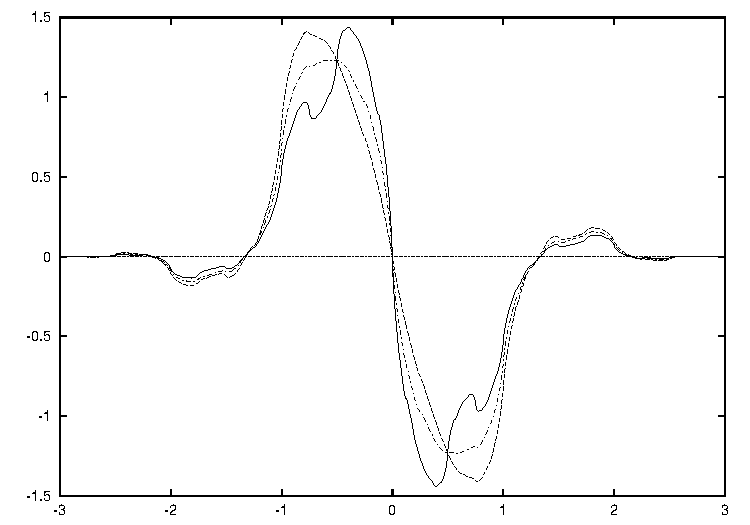
\includegraphics{firstderivative_fund_-0_2_0_15_0}} \par}


\caption{\label{Figdifffund}Derivatives of the fundamental functions for
\protect\( \alpha =-0.2\protect \) (continuous line), \protect\( \alpha =0\protect \)
(dash-dot line), and \protect\( \alpha =0.15\protect \) (dashed line).
The fundamental functions are defined as the interpolation of \protect\( y_{0,k}=\delta _{k,0}\protect \)
by the high resolution subdivision scheme initialized with the \protect\( 4-\protect \)point
Deslauriers-Dubuc dyadic scheme. Derivatives were estimated using
first-order forward finite differences after 8 iterations of the high
resolution scheme (discarding the placeholders at the last iteration).
The \protect\( \alpha =0\protect \) case is in fact the derivative
of the Deslauriers-Dubuc fundamental function.}
\end{figure}

\begin{figure}
{\centering \resizebox*{0.5\textwidth}{!}{\rotatebox{270}{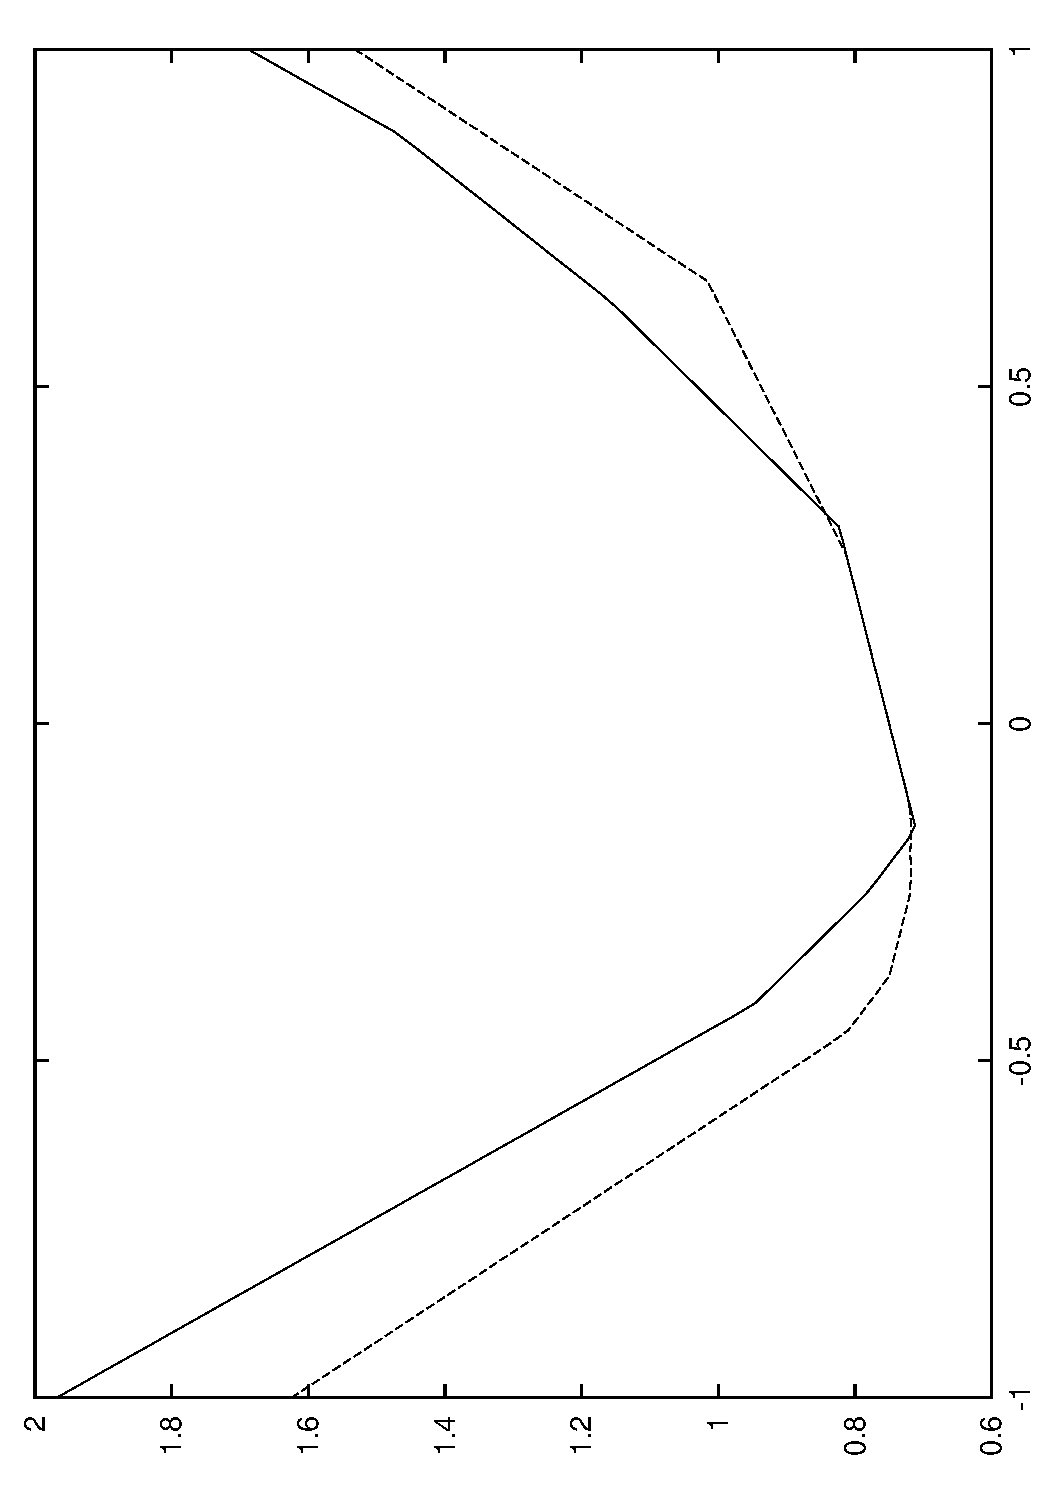
\includegraphics{lambdas}}} \par}


\caption{\label{FigLambdas}\protect\( \lambda _{1}\protect \) (continuous
line) and \protect\( \lambda _{2}\protect \) (dashed line) as functions
of \protect\( \alpha \protect \) (see proof of theorem \ref{maintheorem})
defined as \protect\( \lambda _{1}=\left\Vert 2z^{2}\Gamma _{1}(z)/\left( 1+z\right) ^{2})\right\Vert _{\sum }\protect \)and
\protect\( \lambda _{2}=\left\Vert 2z^{2}(1-z)^{2}\Gamma _{2}(z)/\left( 1+z^{2}\right) ^{2}2z^{2}\Gamma _{1}(z)/\left( 1+z\right) ^{2})\right\Vert _{\sum }\protect \).
The high resolution scheme is differentiable if \protect\( \lambda _{HR}=\max \left\{ \lambda _{1},\lambda _{2}\right\} <1\protect \).}
\end{figure}
Proposition: cubic order of approx. for any \( \alpha  \)

Proposition: For \( \alpha  \), the fundamental function of the high
resolution scheme has values of amplitude <fds for \( |x|>1 \) whereas
the cubic Deslauriers-Dubuc scheme reaches a maximum of .

\begin{thebibliography}{10}
\bibitem{Dau}I. Daubechies, Orthonormal bases of compactly supported wavelets,
Comm. Pure \& Appl. Math. 41, pp. 909--996, 1988.
\bibitem{DeDu}G. Deslauriers and S. Dubuc, Symmetric iterative interpolation processes,
Constr. Approx., 5:49-68, 1989.
\bibitem{DeDuLe}G. Deslauriers, S. Dubuc et D. Lemire, Une famille d'ondelettes biorthogonales
sur l'intervalle obtenue par un sch�ma d'interpolation it�rative,
Ann. Sci. Math. Qu�bec 23 (1999), no. 1, 37-48.
\bibitem{Du}S. Dubuc, Interpolation through an iterative scheme, J. Math. Anal.
Appl., 114:185-204,1986.
\bibitem{DuLeMe}S. Dubuc, D. Lemire, J.-L. Merrien, Fourier analysis of 2-point Hermite
interpolatory subdivision schemes, J. of Fourier Anal. Appl., 7 no.
5, 2001.
\bibitem{Dyn}N. Dyn, Subdivision schemes in computer-aided geometric design, Advances
in numerical analysis (W. Light, ed.), vol. 2, Clarendon Press, 1992,
pp. 36-104.
\bibitem{DyGrLe}N. Dyn, J.A. Gregory, and D. Levin, A 4-point interpolatory subdivision
scheme for curve design. Comput. Aided Geom. Design, 4:257-268, 1987.
\bibitem{KuVD98}F. Kuijt and R.M.J. Van Damme, \emph{Stability of subdivision schemes},
Memorandum No. 1469, Faculty of Mathematical Sciences, University
of Twente, November 1998.
\bibitem{Me92}J.-L. Merrien, A family of Hermite interpolants by bissection algorithms.
Numer. Algorithms 2 (1992) 187-200.
\bibitem{Me99}J.-L. Merrien, Interpolants d'Hermite \( C^{2} \) obtenus par subdivision.
M2An Math. Model. Numer. Anal. 33 (1999) 55-65.\end{thebibliography}

\end{document}
